
\section{Learning actor appearance}


In a sense, poking provides the robot with an operational definition
of what objects are
%% (``things that move when poked'') 
by giving it an
effective procedure for learning about them.  It is not perfect -- for
example, the robot is effectively blind to objects that are too small
or too large -- but for objects at an appropriate scale for
manipulation, it works well.
Once the robot is familiar with a set of such objects,
%Once the robot is familiar with a set of objects in its environment
%that are the right scale for it to manipulate, 
we can go further and provide an operational definition of a {\em
manipulator} as something that acts upon these objects.  We can create
an effective procedure for learning about manipulators by simply
giving the robot a predisposition to fixate familiar objects.  This
enables the same machinery developed for active segmentation to
operate when a foreign manipulator (such as the human hand) pokes the
fixated object.  Of course the robot can easily distinguish
segmentations of its own arm from that of others simply by checking
whether it was commanding its arm to move towards the target at the
time.  The manipulator can be segmented in a manner similar to 
that discussed in Section~\ref{sect:poking}.
%by hypothesizing that it moves
%towards the object at a constant velocity in the period immediately
%preceding the moment of contact.  
%Estimating the velocity from the
%gross apparent motion allows the segmentation problem to be expressed
%in the form introduced in Section~\ref{sect:min-cut}, 
%where the
%foreground is now taken to be regions moving at the desired velocity,
%and the background is everything else.
Figure~\ref{fig:auto-proto-flipper}
shows results for this procedure.  The results are based on
relatively little data, yet are already
sufficient to pick out good prototype views for the robot and human
manipulator.
A procedure like this could be used to autonomously
train a recognizer for the human hand, which could then
be included in further operational definitions, expanding
the robot's domain of grounded knowledge ever outwards.

\begin{figure}[tb]
\begin{center}
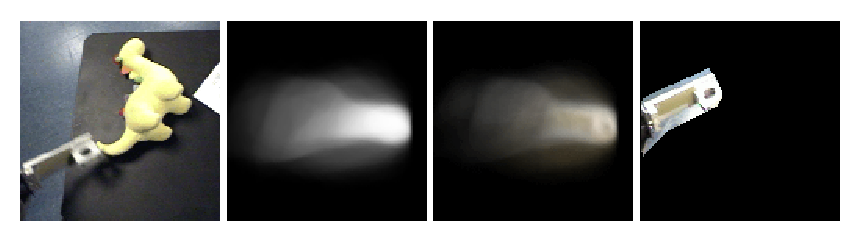
\includegraphics[width=\columnwidth]{fig-auto-proto-flipper.eps}\\
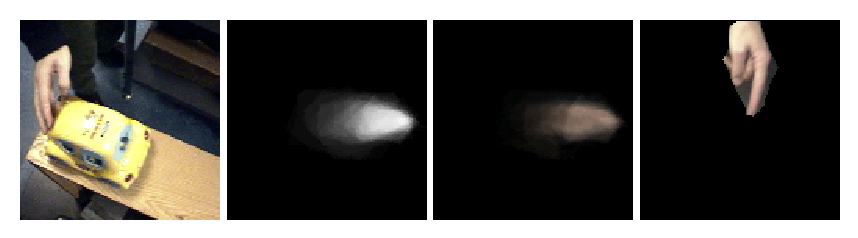
\includegraphics[width=\columnwidth]{fig-auto-proto-hand.eps}
\caption{ 
\label{fig:auto-proto-flipper}
%
The robot manipulator (top left) was automatically segmented during 20
poking sequences.  The segmentations were aligned and averaged, giving
the mask and appearance shown in the adjacent images.  The best
matching view is shown on the top right.  A similar result for the
human hand is shown on the bottom, based on much less data (5 poking
sequences, hands of two individuals).
%BREAK
%The human hand (see left) was automatically segmented during just 5
%poking sequences.  Hands of two different individuals were used.  The
%segmentations were aligned and averaged, giving the mask shown in the
%second image and the mean view shown in the third.  The best matching
%view is shown on the right.  
%Despite the paucity of the data,
%the mean view at least captures skin tone, which is sufficient to
%discard poor segmentations from consideration.
%
}
\end{center}
\end{figure}

